\documentclass{beamer}


\usepackage[utf8]{inputenc}
\usepackage{amsmath}
\usepackage{amsfonts}
\usepackage{amssymb}
\usepackage{graphicx}
\usepackage{ragged2e}  % `\justifying` text
\usepackage{booktabs}  % Tables
\usepackage{tabularx}
\usepackage{tikz}      % Diagrams
\usetikzlibrary{calc, shapes, backgrounds}
\usepackage{amsmath}
\usepackage{amssymb}
\usepackage{dsfont}
\usepackage{url}       % `\url
\usepackage{listings}  % Code listings
\usepackage[T1]{fontenc}
\usepackage[percent]{overpic}
\usetikzlibrary{trees}
\usepackage[absolute,overlay]{textpos}
\usepackage{tcolorbox}



\newtcolorbox{terminal}{colback=black!70!white,colframe=black!70!white}
\newtcolorbox{focus}{colback=black!10!white,colframe=black!10!white}

\usepackage{theme/beamerthemehbrs}

\author[MAS]{Hassan Umari}
\title{ROS Nodes, Topics, and Messages}
\subtitle{Foundation Course}
\institute[HBRS]{Hochschule Bonn-Rhein-Sieg}
\date{\today}
\subject{ROS workshop}

% \thirdpartylogo{path/to/your/image}


\begin{document}
{
\begin{frame}
\titlepage
\end{frame}
}


\section{Recap}
\begin{frame}{Recap}
    \framesubtitle{Summary of yesterday's session}
    \begin{itemize}
        \item ROS is a collection of libraries and tools that helps you when you develop software for robots.
              
        \item ROS provides several ways to transfer data between nodes:
        
        \begin{enumerate}
            \item ROS topics and messages (\textbf{publish/subscribe}).
            \item ROS services (\textbf{request/reply}).
            \item ROS actions (\textbf{request/reply}).
            \item Parameter server.
        \end{enumerate}   
    \end{itemize}
\end{frame}


\begin{frame}{Recap}
    \framesubtitle{Summary of yesterday's session}
    \begin{itemize}
        \item We will focus today on ROS topics and messages..
    \end{itemize}
\end{frame}


     \begin{frame}[plain]{}
         \centering
         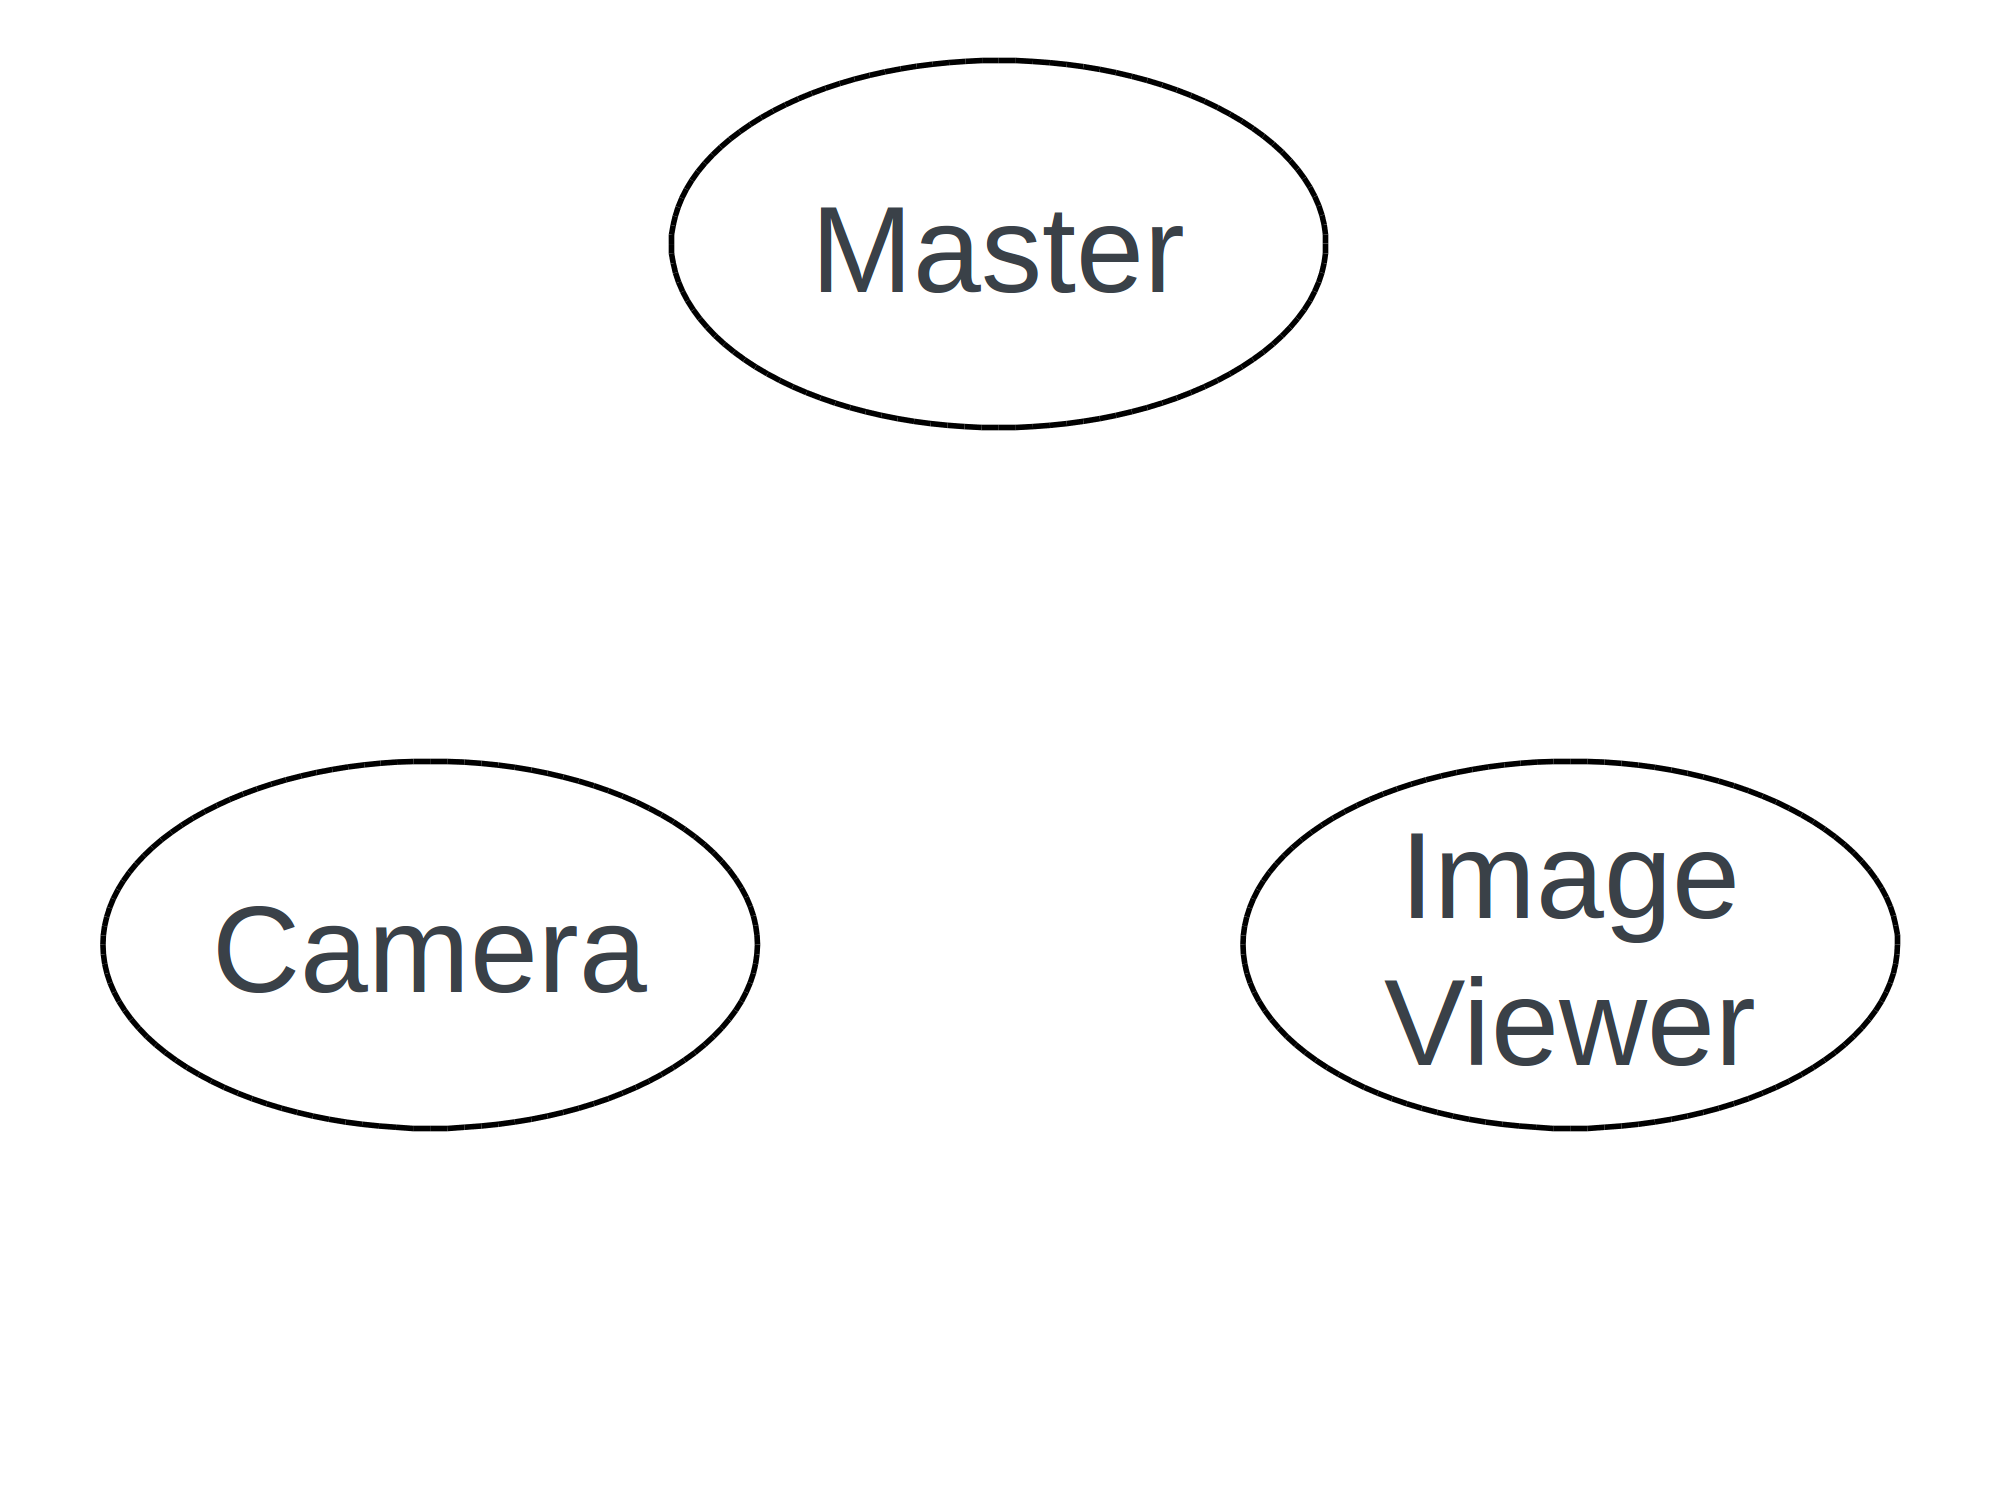
\includegraphics[width =1.0\linewidth]{figures/master1.png}                                                              
        \end{frame} 
        \begin{frame}[plain]{}
            \centering
            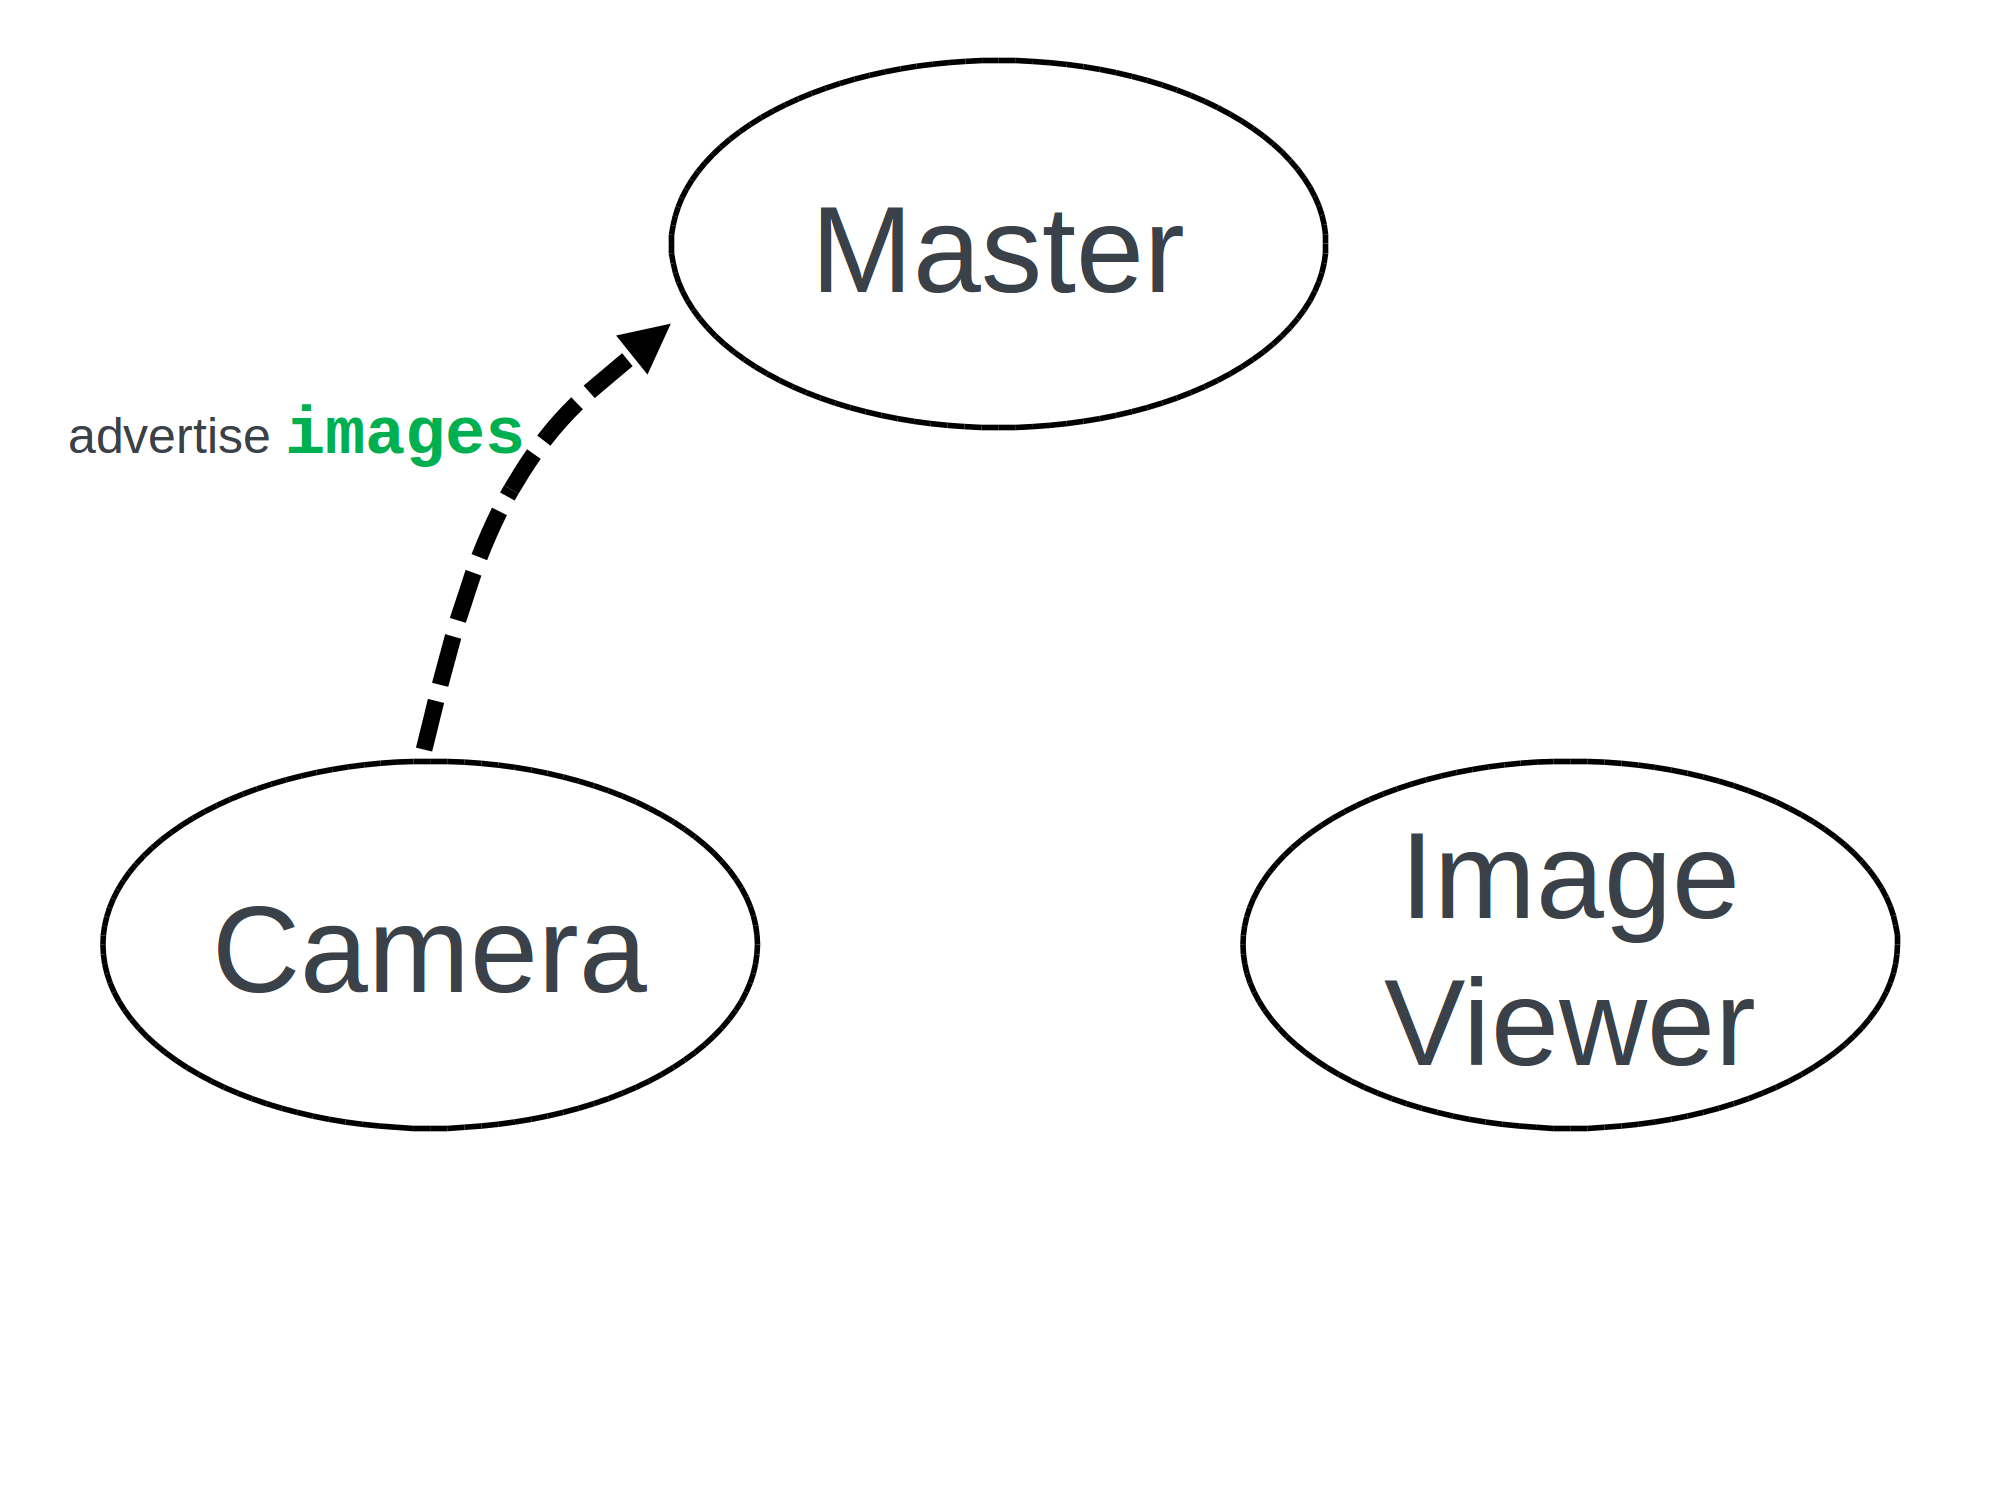
\includegraphics[width =1.0\linewidth]{figures/master2.png}                                                              
        \end{frame} 
        \begin{frame}[plain]{}
            \centering
            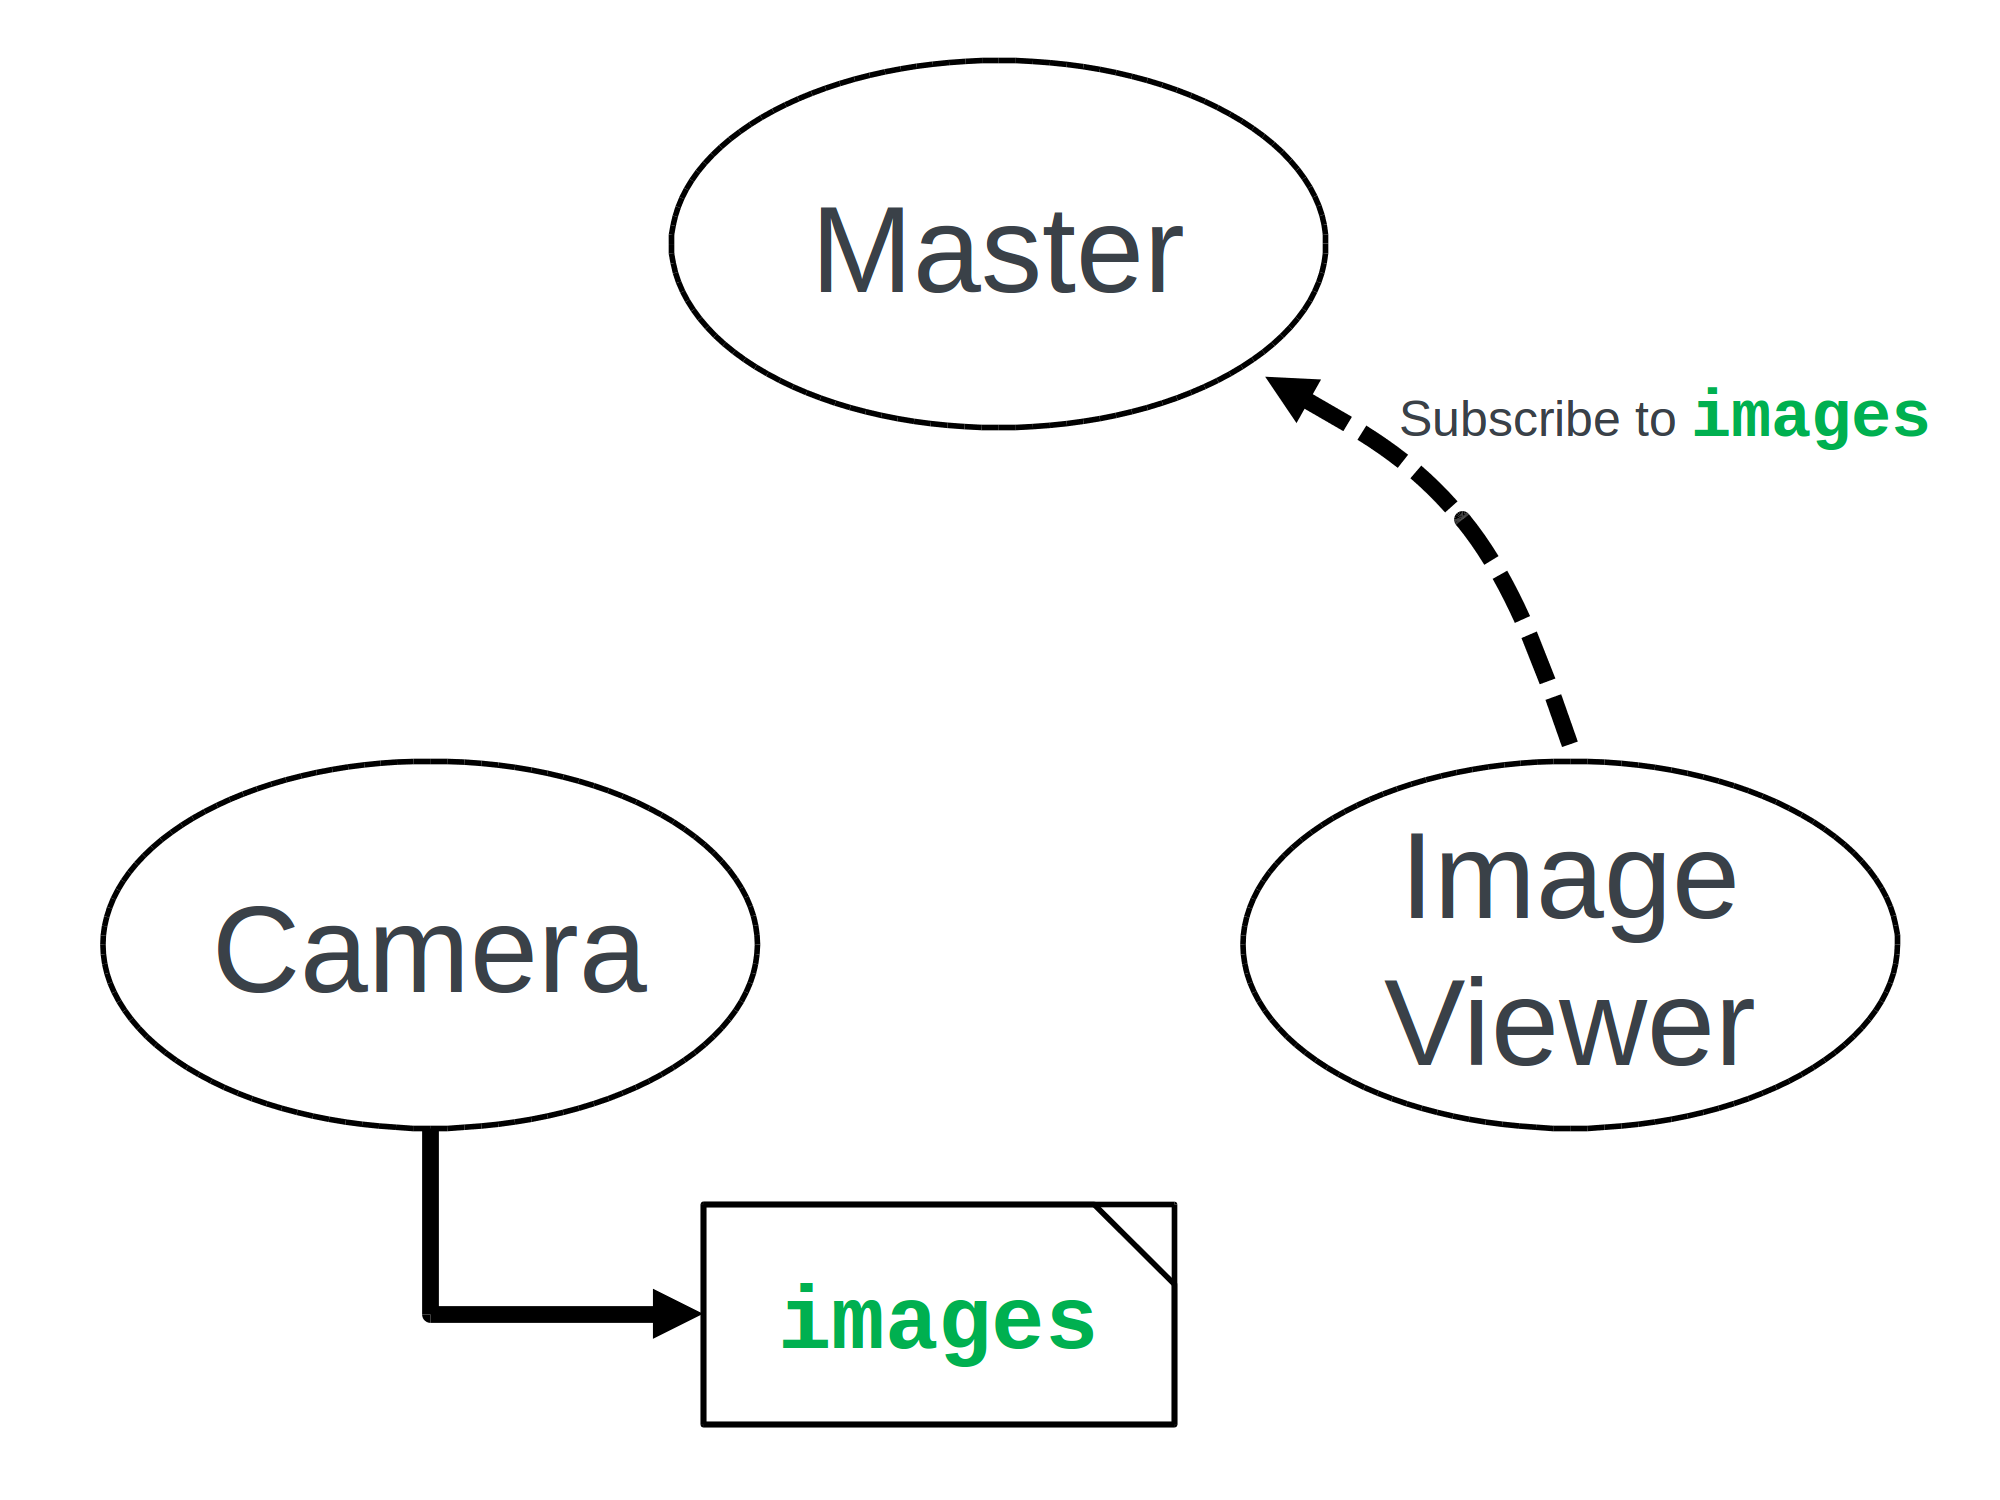
\includegraphics[width =1.0\linewidth]{figures/master3.png}                                                              
        \end{frame} 
        \begin{frame}[plain]{}
            \centering
            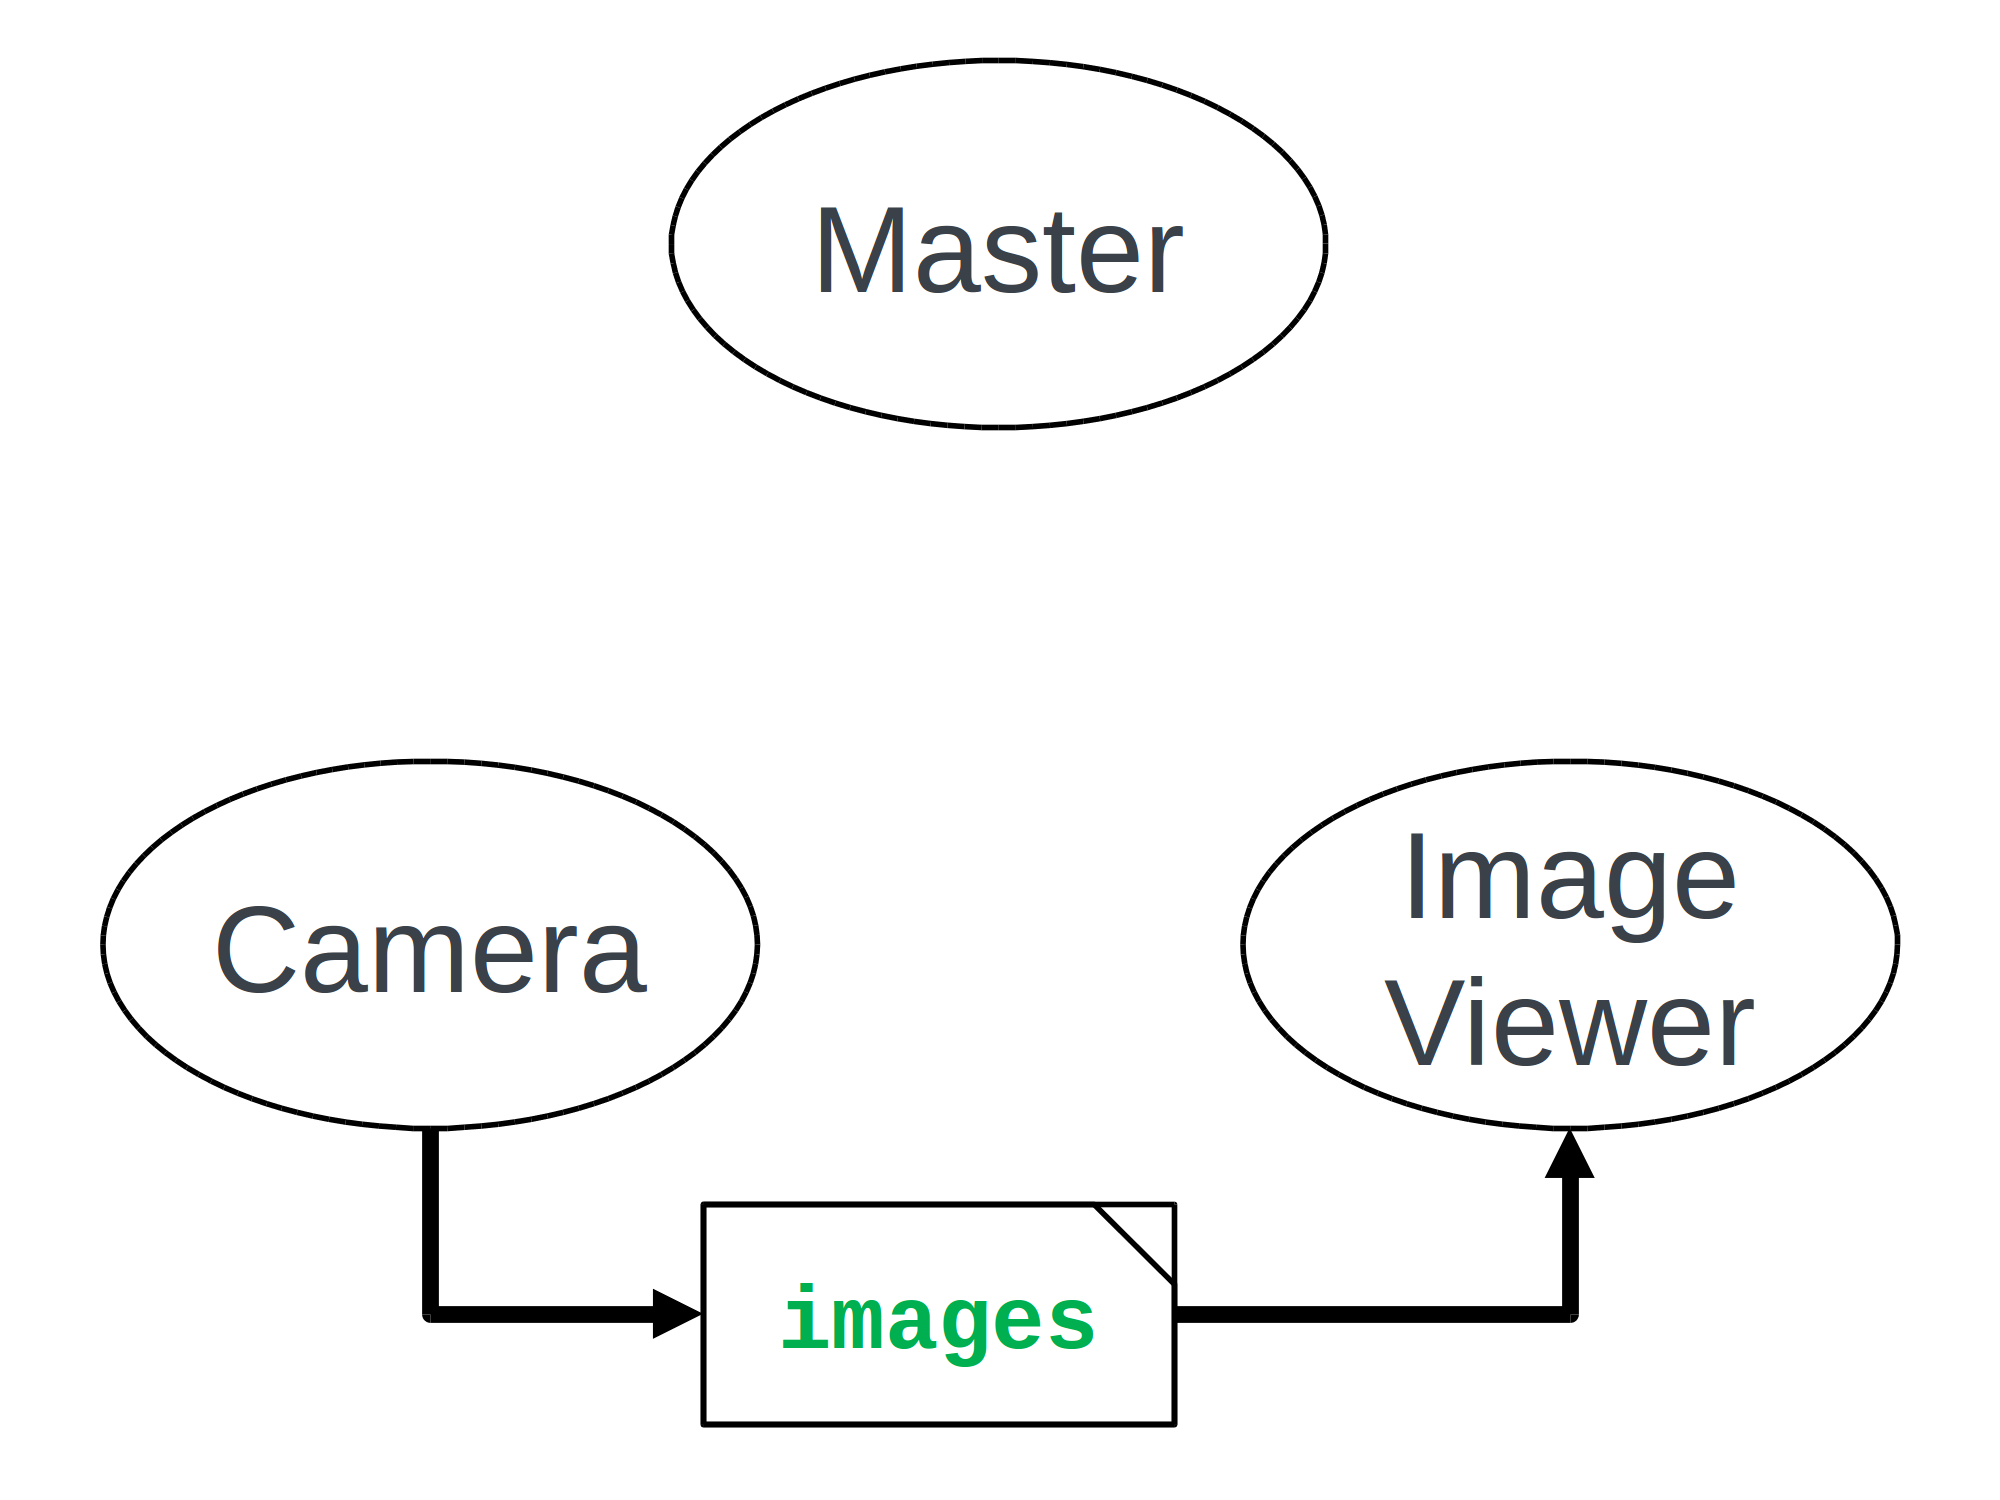
\includegraphics[width =1.0\linewidth]{figures/master4.png}                                                              
        \end{frame}
        
        

        
\section{ROS nodes in Python}

\subsection{A simple ROS node in Python}

\begin{frame}[fragile]{A simple ROS node}
    \framesubtitle{   ../scripts/00\_simple\_node.py}
    \lstset{language=python,
        basicstyle=\ttfamily,
        keywordstyle=\color{blue}\ttfamily,
        stringstyle=\color{red}\ttfamily,
        commentstyle=\color{green}\ttfamily,
        morecomment=[l][\color{magenta}]{\#},
        showstringspaces=false
    }
    \begin{lstlisting}
#!/usr/bin/env python


import rospy
from time import sleep

rospy.init_node("print_text")


while True:
    print "Hello world!"
    sleep(1)
    \end{lstlisting}
\end{frame}



\begin{frame}[fragile]{A simple ROS node}
    \framesubtitle{   ../scripts/01\_simple\_node.py}
    \lstset{language=python,
        basicstyle=\ttfamily,
        keywordstyle=\color{blue}\ttfamily,
        stringstyle=\color{red}\ttfamily,
        commentstyle=\color{green}\ttfamily,
        morecomment=[l][\color{magenta}]{\#},
        showstringspaces=false
    }
\begin{lstlisting}
#!/usr/bin/env python

import rospy


rospy.init_node("print_text")  
rate = rospy.Rate(1)

while not rospy.is_shutdown():
    print "Hello world!"
    rate.sleep()
\end{lstlisting}
\end{frame}



\begin{frame}[fragile]{Writing a publisher node in Python}
    \framesubtitle{../scripts/02\_simple\_publisher.py}
    \begin{focus}
        \centering
        \fontsize{9}{1} \ttfamily rospy.init\_node({\color{blue}'node name'})
    \end{focus}
    
    \begin{itemize}
        \item nodes name must be unique. If you want to make sure the name of the node is unique:
        
        
        \begin{focus}
            \centering
            \fontsize{9}{1} \ttfamily rospy.init\_node({\color{blue}'node name'}, anonymous= {\color{blue}True})
        \end{focus}
        \item node name will look like this: \ttfamily /print\_text\_19637\_1567065017476
    \end{itemize}
    
\end{frame}



\begin{frame}{Three ways to run a node}
    \framesubtitle{ROS Nodes}
    
    There are 3 ways to run a node:
    \begin{enumerate}
        \item Like you normally do {\tiny{(not recommended)}}. Example (in case of python node):
                \begin{terminal}
                \color{green} \ttfamily{python <file name>}
                \end{terminal}
        \item using rosrun command:
        \begin{terminal}
        \color{green} \ttfamily{rosrun <package name> <node name>}
        \end{terminal}
        
        \item Using launch files. \tiny{(we'll see it later)}

    \end{enumerate}
\end{frame}

\begin{frame}{Let's create a package first!}
    \framesubtitle{ROS Nodes}
\begin{itemize}
    \item ROS commands find your files (python scripts, cpp files, launch files, message definitions) if they are located in a package inside the workspace.
    
    \item Normally, a package looks like this:
 
\end{itemize}

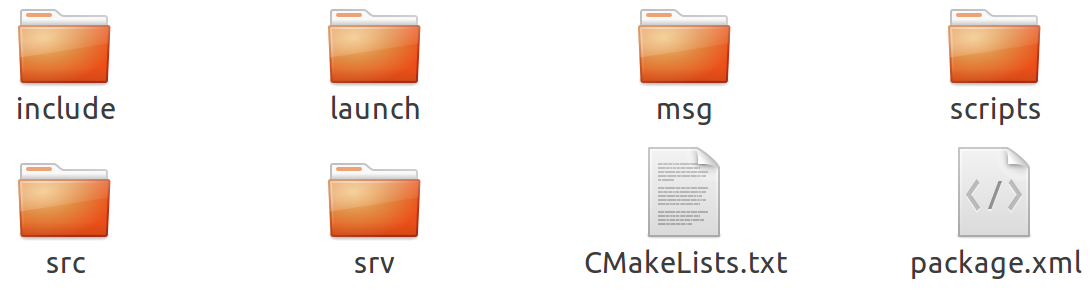
\includegraphics[width = 1\linewidth]{figures/package.png}

\end{frame}

\begin{frame}{Let's create a package first!}
    \framesubtitle{ROS Nodes}

    \begin{itemize}
        \item  go to the README and do the steps for \textbf{creating a package}. 
    \end{itemize}   
\end{frame}


\begin{frame}{ROS commands}
    \framesubtitle{ROS Nodes}
\begin{itemize}
    \item Navigate to a ROS package directly:

    \begin{terminal}
        \color{green} \ttfamily{roscd <package name>}
    \end{terminal}
    
    \item run a node without navigating to it's directory:

    \begin{terminal}
        \color{green} \ttfamily{rosrun <package name> <executable>}
    \end{terminal}
\end{itemize}

\end{frame}


\begin{frame}{Let's create a package first!}
    \framesubtitle{ROS Nodes}
    
    \begin{itemize}
        \item  go to the README and do the steps for \textbf{running a node}. 
    \end{itemize}   
\end{frame}


\begin{frame}{More ROS commands}
    \framesubtitle{ROS Nodes, Topics, and Messages}
    \begin{itemize}
        \item List all the running nodes::
        
        \begin{terminal}
            \color{green} \ttfamily{rosnode list}
        \end{terminal}
        
        \item Get more info. about a certain node:
        
        \begin{terminal}
            \color{green} \ttfamily{rosnode info <node name>}
        \end{terminal}
        
              
        
    \end{itemize}
    
\end{frame}


\subsection{Writing a publisher node in Python}

\begin{frame}[fragile]{Writing a publisher node in Python}
    \framesubtitle{ROS Nodes, Topics, and Messages}
    
    \begin{itemize}
        \item  Let's extend our previous node and make it publish a String ROS message.
    \end{itemize}   
\end{frame}
 
\begin{frame}[fragile]{Writing a publisher node in Python}
    \framesubtitle{../scripts/02\_simple\_publisher.py}
    

                   
    \lstset{language=python,
        basicstyle=\scriptsize,
        keywordstyle=\color{blue}\ttfamily,
        stringstyle=\color{red}\ttfamily,
        commentstyle=\color{green}\ttfamily,
        morecomment=[l][\color{magenta}]{\#},
        showstringspaces=false
    }
\begin{lstlisting}
#!/usr/bin/env python

import rospy

from std_msgs.msg import String

rospy.init_node('talker')

pub = rospy.Publisher('myFirstTopic', String, queue_size=10)

rate = rospy.Rate(1)

my_message = String()
my_message.data = "Hello there! How are you?"

while not rospy.is_shutdown():
    pub.publish(my_message)
    rate.sleep()
\end{lstlisting}
\end{frame}




\begin{frame}[fragile]{Writing a publisher node in Python}
    \framesubtitle{../scripts/02\_simple\_publisher.py}
    \begin{focus}
        \centering
        \fontsize{9}{1} \ttfamily rospy.Publisher({\color{blue}name}, {\color{blue}data\_class}, {\color{blue}queue\_size})
    \end{focus}
    
    \begin{itemize}
        \item {\ttfamily name}: Name of the topic to publish on.
        
        \item {\ttfamily data\_class}: The type of message. It is a ROS message class.
        
        \item {\ttfamily queue\_size}: The size of the outgoing message queue.
        
    \end{itemize}
\end{frame}

\begin{frame}[fragile]{Writing a publisher node in Python}
    \framesubtitle{../scripts/02\_simple\_publisher.py}
    \begin{focus}
        
        \ttfamily rospy.Publisher(\\
                                 {\color{red}name},\\
                                 {\color{red}data\_class},\\
                                 {\color{blue}subscriber\_listener=None}, \\
                                 {\color{blue}tcp\_nodelay=False},\\
                                 {\color{blue}latch=False},\\
                                 {\color{blue}headers=None},\\
                                 {\color{red}queue\_size=None}\\)
    \end{focus}

\end{frame}


\begin{frame}[fragile]{Writing a publisher node in Python}
    \framesubtitle{Things to note..}
    
    \begin{itemize}
        \item  ROS messages are implemented as classes.
        \item  To publish a message you also need to define a \textbf{Publisher} class.
        \item Most of ROS concepts and functionalities are implemented as classes. This is why understanding OOP helps you understand ROS better.
    \end{itemize}   
\end{frame}


\begin{frame}[fragile]{Writing a publisher node in Python}
    \framesubtitle{ROS Nodes, Topics, and Messages}
    
    \begin{itemize}
        \centering
        \item  Go to the README file and do the instructions of section: \textbf{some of ROS commands}.
    \end{itemize}   
\end{frame}




\begin{frame}{More ROS commands}
    \framesubtitle{ROS Nodes, Topics, and Messages}
    \begin{itemize}
        \item Get the current list of topics:
        
        \begin{terminal}
            \color{green} \ttfamily{rostopic list}
        \end{terminal}
        
        \item Print published messages:
        
        \begin{terminal}
            \color{green} \ttfamily{rostopic echo <topic name>}
        \end{terminal}
        
        
        \item Get message type of a topic:
        
        \begin{terminal}
            \color{green} \ttfamily{rostopic type <topic name>}
        \end{terminal}
  
  
    \end{itemize}
    
\end{frame}




\subsection{How to use ROS messages}

\begin{frame}{How to use ROS messages}
    \framesubtitle{ROS Nodes, Topics, and Messages}
    \begin{itemize}
        \item ROS messages are just classes with attributes you can fill.
        
        \item ROS messages are defined in a separate files and have to be placed in a package. (will be covered today).
        
        \item The following command can be used to see the class attributes, or the description, of a ROS message:
        
        \begin{terminal}
            \color{green} \ttfamily{rosmsg show <package/msg>}
        \end{terminal}
    \end{itemize}
    
\end{frame}


\begin{frame}{How to use ROS messages}
    \framesubtitle{Example}

        \begin{terminal}
            \color{green} \ttfamily{rosmsg show std\_msgs/String }
        \end{terminal}

    The output is:
    
            \begin{terminal}
                \color{green} \ttfamily{string data}
                
            \end{terminal}
   
   \begin{itemize}
       \item It means ROS {\ttfamily \colorbox{yellow}{String}} message is a class with an attribute named {\ttfamily \colorbox{yellow}{data}} of type string (Python string).
   \end{itemize} 
\end{frame}


\begin{frame}{How to use ROS messages}
    \framesubtitle{Importing a ROS message}
    
    
    \begin{itemize}
        \item {\ttfamily \colorbox{yellow}{String}} message is located in the {\ttfamily \colorbox{yellow}{std\_msgs}}.
    \end{itemize} 
\end{frame}



\begin{frame}[plain]{}
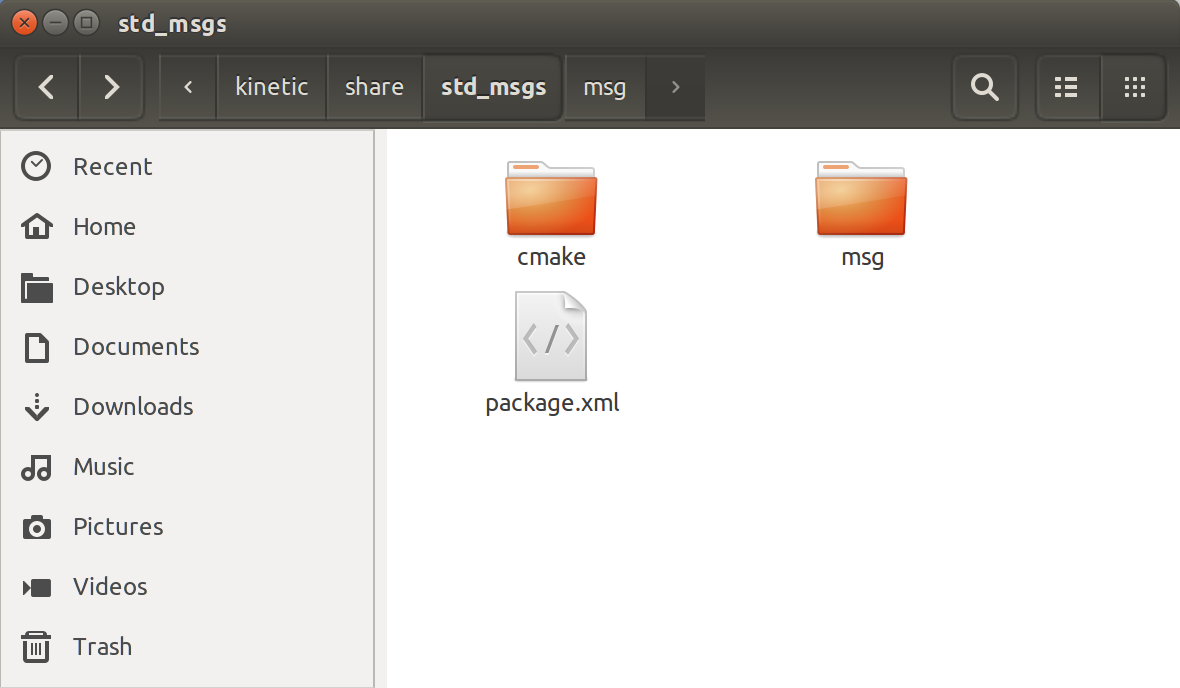
\includegraphics[width=1.0\linewidth]{figures/std_msgs.png}
\end{frame}

\begin{frame}[plain]{}
    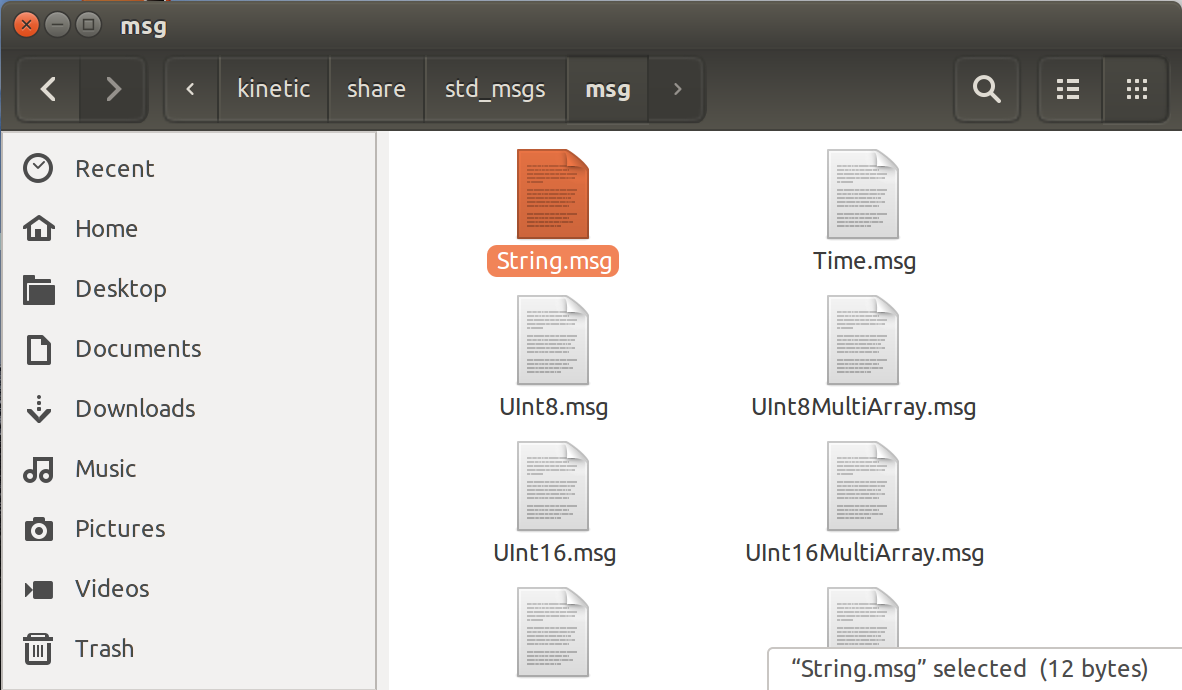
\includegraphics[width=1.0\linewidth]{figures/string.png}
\end{frame}




\begin{frame}[fragile]{How to use ROS messages}
    \framesubtitle{Importing a ROS message}
    \lstset{language=python,
        basicstyle=\ttfamily,
        keywordstyle=\color{blue}\ttfamily,
        stringstyle=\color{red}\ttfamily,
        commentstyle=\color{green}\ttfamily,
        morecomment=[l][\color{magenta}]{\#},
        showstringspaces=false
    }
    \begin{lstlisting}

    
    from std_msgs.msg import String

    \end{lstlisting}
\end{frame}








\subsection{Writing a subscriber node in Python}

\begin{frame}[fragile]{Writing a subscriber node in Python}
    \framesubtitle{ROS Nodes, Topics, and Messages}
    
    \begin{itemize}
        \item  Let's ..
    \end{itemize}   
\end{frame}

\begin{frame}[fragile]{Writing a publisher node in Python}
    \framesubtitle{../scripts/02\_simple\_publisher.py}
    
    
    
    \lstset{language=python,
        basicstyle=\scriptsize,
        keywordstyle=\color{blue}\ttfamily,
        stringstyle=\color{red}\ttfamily,
        commentstyle=\color{green}\ttfamily,
        morecomment=[l][\color{magenta}]{\#},
        showstringspaces=false
    }
    \begin{lstlisting}

    \end{lstlisting}
\end{frame}











\section{ROS messages}
    

\begin{frame}[fragile]{rospy reference}
    \framesubtitle{}

\begin{itemize}
    \item rospy full documentation (all the classes, all the functions ..etc):
    
    \vspace{0.5cm}
     \url{http://docs.ros.org/kinetic/api/rospy/html/}
\end{itemize}
    
\end{frame}





\end{document}
